The detection method can be divided into the following three steps:
\begin{enumerate}
  \item Preliminary segmentation
  \item Ball probability estimation
  \item Best candidates selection
\end{enumerate}

Preliminary segmentation is performed to decrease the ROI from the entire table area to areas that contains balls.

In step 2 the ROI is traversed, and a ball probability is computed at each possible ball location. 

To establish which of the positions inside the ROI are actual ball positions, the balls are selected from the list of probabilities starting with the most probable position.

\subsection{Preliminary Segmentation}
To decrease the ROI from the cloth area down to areas of the table that contains balls, a preliminary segmentation is performed. A color threshold removes all pixels that belong to the background leaving behind a mask that represents the balls.
\begin{figure}[htpb]
  \centering
  \subfloat[Original]{\label{fig:gull}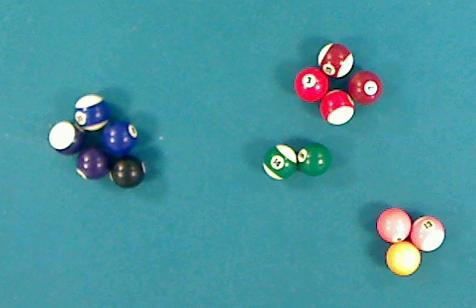
\includegraphics[width=0.48\textwidth]{images/thres1before.jpg}}
  \quad           
  \subfloat[Segmentation]{\label{fig:tiger}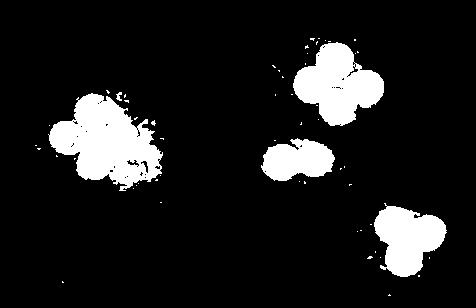
\includegraphics[width=0.48\textwidth]{images/thres1after.jpg}}
   \caption{Color threshold to remove background}
  \label{fig:thres1}
\end{figure}
Figure \ref{fig:thres1} shows the result of the color threshold. In a situation like this where the balls are laying close to each other, the preliminary segmentation is not enough to successfully separate the balls. Balls in close proximity results in connected BLOBs after the threshold. These BLOBs could be separated using morphology operations but most of the information would be lost, causing the locations to lack precision. Instead of using the BLOBS directly, they are used as search regions for the balls.

\subsection{Ball Probability Estimation}
To be able to estimate the ball probability, we need to know the features that characterizes a ball. The following description can be formulated:
\begin{itemize}
\item The shape of the ball, in the image, is always a circle of fixed size
\item The color distribution consists of at least two of three parts:
	\begin{itemize}
		\item White
		\item Black (ball number)
		\item Primary ball color
	\end{itemize}
\end{itemize}
The black and cue balls has black and white, respectively, as their primary color, making them consist of only two distributions, whereas all other balls consists of three. This ball description allows us to formulate a measure for the probability that a given position in the image corresponds to the center of a ball.

If we ignore the black pixels from the ball number, the balls does only contain one primary color and white. A candidate ball position is defined as a circular ROI in the image having position the the center of the ROI circle.
The probability of a candidate position containing a ball can then be formulated as the ratio between the number of pixels in the ROI following this rule and the total pixels:
\begin{equation}
P_{ball}(x,y) = \frac{pixels_{primary} + pixels_{white}}{pixels_{total}}
\end{equation}
It is seen that the a region having only one color besides white maximizes the probability.
\begin{figure}[htpb]
\begin{center}
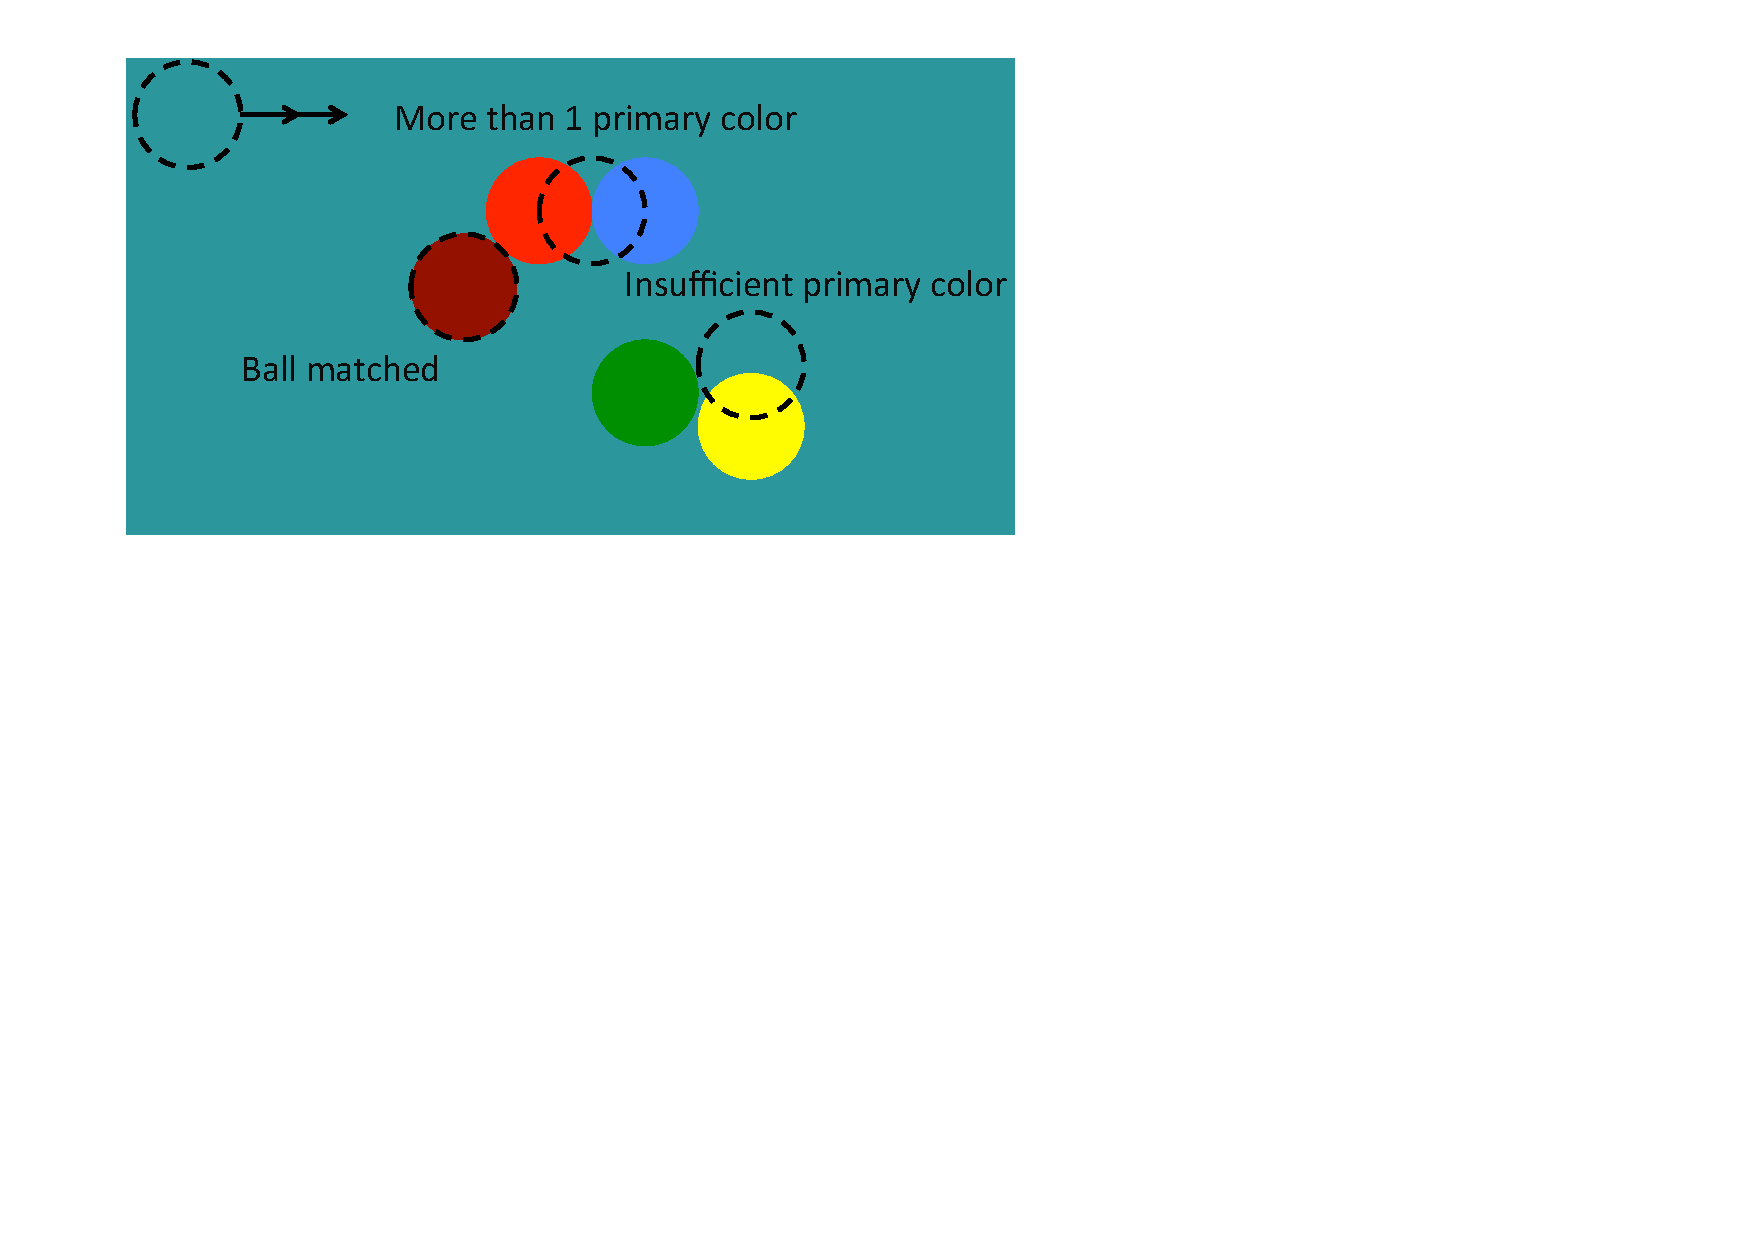
\includegraphics[width=0.8\textwidth]{images/ballfind.pdf}
\caption{The probability of a ball is evaluated in the image.}
\label{fig:ballfind}
\end{center}
\end{figure}
Figure \ref{fig:ballfind} shows the process of computing the ball probability. The probability is computed in every possible ball position.
A circular mask is placed in every position found by the preliminary segmentation. By using a circular mask, the system is able to get a better match against the circular ball regions. Inside the mask an HSB color histogram is computed. All pixels that have a hue value close to the background hue are ignored. The rest of the pixels are sorted into three categories: 
\begin{enumerate}
  \item White pixels
  \item Black pixels
  \item Colored pixels
\end{enumerate}
Pixels that have a saturation below a certain value are considered to be white. Pixels with brightness below a threshold are considered to be black. To make the system as color independent as possible, brightness is only used to identify black pixels. This is necessary because the black color is undefined in hue-saturation space. For further information see section \ref{sec:analballs} concerning analysis of ball color.

To determine the number of primary colored pixels, the variance of the colored pixels is analyzed. If the candidate position contains a ball, the distribution of the colored pixels is expected to be narrowly distributed around the mean of the ball color. If the position is between two or more balls the distribution will be multimodal and the variance higher.

The pixels that are within a certain deviation of the mean hue are counted, resulting in a count of the number of primary colored pixels in the ball.

If the number of black pixels is greater than the number of primary colored pixels, the number of black pixels is used as the number of primary pixels.
\subsection{Best Candidates Selection}
The result of the probability estimation is a sorted list of candidate positions, having the most probable position at the top of the list. The probability has been computed in every image position, which results in many overlapping positions. 

The final ball positions are found by traversing the list from the top and thus selecting the most probable positions first. A candidate will only be selected if there is not already a detected ball one radius of the candidate position.  

The system continues to detect balls until 16 balls are found or the score is below a threshold. This threshold is set as a ratio of the total pixels in a ball. The whole process can be seen in figure \ref{fig:ballflowchart}.

\fxnote{Figure showing different distributions and their resulting ball probability}
\begin{figure}[htpb]
\begin{center}
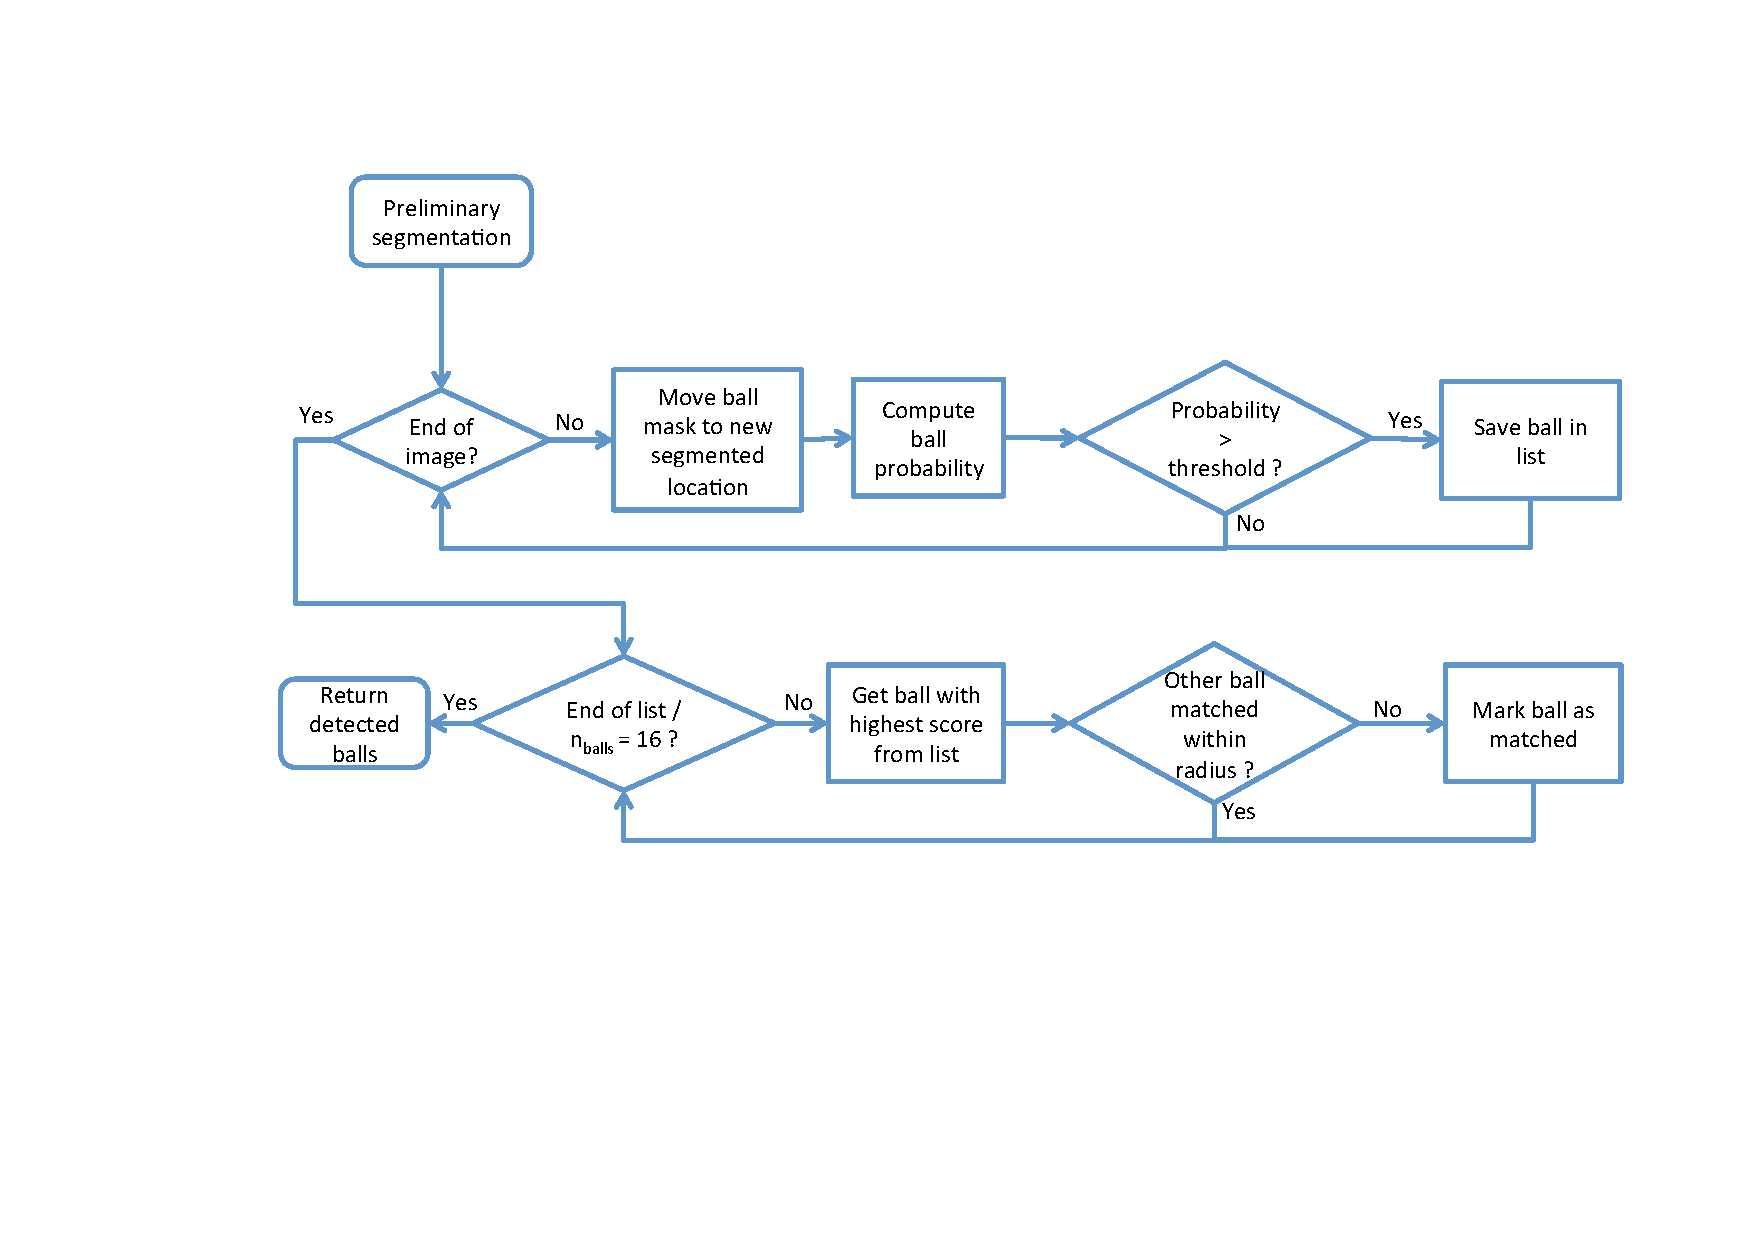
\includegraphics[width=\textwidth]{images/ballflowchart.pdf}
\caption{Flowchart of the ball detection process.}
\label{fig:ballflowchart}
\end{center}
\end{figure}

A problem arises if a wrong match is found, which intersects candidates that have not yet been matched. The position of the intersected candidates will then be invalidated, because they are within the radius of a detected ball. It will then be impossible to find a new match in the region of the earlier wrong match. 
\begin{figure}[htpb]
\begin{center}
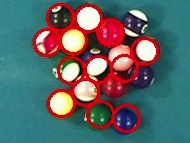
\includegraphics{images/wronglocate.jpg}
\caption{Consequence of wrong location detection. Red circles are ball detected balls}
\label{fig:wronglocate}
\end{center}
\end{figure}
Figure \ref{fig:wronglocate} shows the problem of a wrong match. The wrong match prevents several balls from being matched, and other balls from matching precisely.

\subsection{Detection Results}
Figure \ref{fig:detect} shows results of ball detection in 2 different situations. The detector shows good performance in uncluttered aswell as cluttered ball arrangements. The cluttered balls does however affect the precision of the detection

\begin{figure}[htpb]
  \centering
  \subfloat[No clutter]{\label{fig:gull}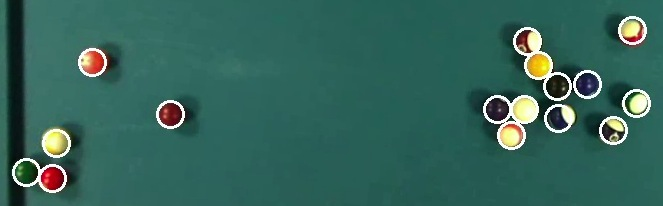
\includegraphics[width=0.48\textwidth]{images/detect1.jpg}}
  \quad           
  \subfloat[Clutter]{\label{fig:tiger}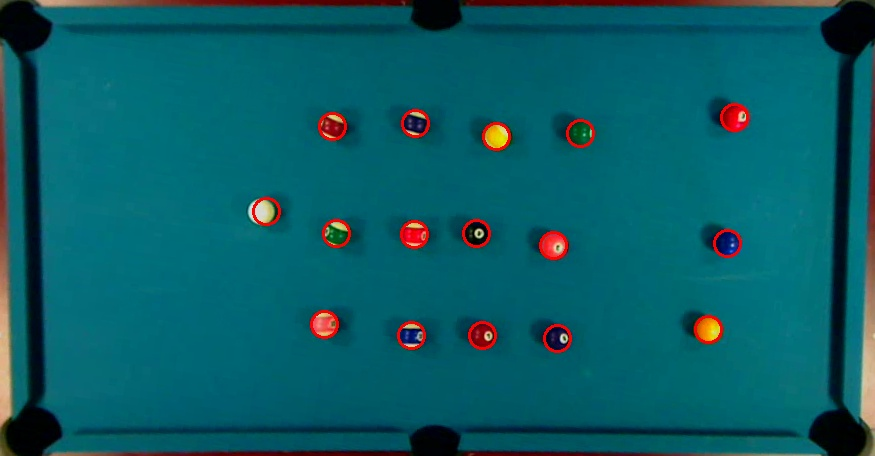
\includegraphics[width=0.48\textwidth]{images/detect2.jpg}}
   \caption{Results of ball detection. White circles indicate detected ball positions.}
  \label{fig:detect}
\end{figure}

